
\chapter{Implementace a testování metod}
\label{chap:impl}

Praktická část práce se zabývá porovnáním výkonnosti jednotlivých
metod nalezení a popisu bodových příznaků na datasetu (JAK CITOVAT DATASET?)

Tento dataset sestává z jednotlivých subsetů obsahujících vždy několik obrázků
zobrazujících jednu scénu pod různými prostorovými transformacemi a porovnává se
vždy jeden z obrázků v subsetu s postupně všemi ostatními. Tyto transformace
lze popsat maticí homografie a dataset ke každému zkoumanému páru nabízí vzorovou
matici homografie.

Na tomto datasetu jsou zkoumány detektory příznakových bodů Harris, GFTT (neboli
Shi-Tomasi), SIFT, SURF, FAST, ORB a MSER a deskriptory BRIEF, SIFT, SURF a ORB.
Body nalezené a popsané těmito algoritmy jsou potom mezi jednotlivými obrazy
přiřazeny a metodou na bázi RANSAC je z nich aproximována matice homografie a 
jsou označeny body (páry bodů), které byly pro tuto aproximaci vzaty jako správné a ty, 
které byly zavrženy jako chybně přiřazené. 

%MĚŘÍTKO KVALITY NALEZENÉ HOMOGRAFIE

Jak bylo zmíněno, ke každému porovnávanému páru obrázků přísluší matice homografie,
která popisuje geometrickou transformaci mezi prvním a druhým obrázkem. Program
pomocí identifikace a spárovnání příznakových bodů s využitím metody RANSAC spočítá
odhad této homografie. Vzdálenost deklarované a nalezené homografie je potom brána
jako měřítko kvality konkrétní metody nebo kombinace metod na daném datasetu. Kvalita
homografie nabývá hodnot od 0 do 100\% a vypočítává se jako:

\begin{align}
	pi_1 = H_1 * eig(H_1) \\
	pi_2 = H_2 * eig(H_2) \\
	dif = pi_1 - pi_2 \\
	100*(\frac{pi}{2} - atan(dif \times{} 10^-4))
\end{align}

kde $H_1$ je homografie deklarovaná v datasetu, $H_2$ je matice homografie nalezená
programem, $eig(H)$ jsou vlastní čísla matice $H$. 

Toto měřítko je v tabulkách ozančeno 'score'. Dále je zkoumán celkový počet přiřazených
bodů (označen 'matches') a z něj počet bodů použitých k aproximaci homografie (označen 'inliers').
Dále jsou zkoumány časy pro detekci a popis při použití jednotlivých detektorů a deskriptorů. 

%IMPLEMENTACE

Porovnání jednotlivých metod bylo implementováno v hlavním programu v C++ s využitím frameworku
openCV. Zpracování datasetu, dávkové spouštění porovnání a statistické vyhodnocení výsledků bylo
implementováno v jazyku Python s využitím knihovny Pandas.

%OBR: PSEUDOUML implementace

Data o souborech v datasetu jsou vytěžena pomocí skriptu \verb|create_configs.py| v Pythonu a zkompilována do konfiguračních souborů pro hlavní program BP. Skript \verb|run_batch.py| poté tyto konfigurační soubory načte a postupně s nimi spustí hlavní program. Ten pro každou vybranou složku datasetu vytvoří výstupní složku s obrázky, které zobrazují nalezené a spojené body mezi jedním a druhým obrázkem z vyhodnocovaného páru a soubor \verb|data.csv|, který obsahuje informace o jednotlivých párech, rychlostech vyhodnocení a kvalitě odhadu homografie. Skript \verb|get_data.py| ze souborů \verb|data.csv| vytvoří jeden globální soubor a několik souborů se subsety podle transformace, kterou reprezentují: Úhel (ve smyslu změna polohy pozorovatele směrem do stran), rotace (okolo osy procházející středem fotoaparátu), zoom, nasvětlení, rozostření a změna rozlišení. Tyto soubory jsou potom zpracovány skriptem \verb|pandas_stats.py| do obrázků a tabulek v této kapitole.

\begin{tabular}{ l l l l }
	 methods & avg matches & avg inliers & avg score [\%] \\
	 Harris -> BRIEF & 482.155844156 & 11.4025974026 & 4.05431356598 \\
	 Harris -> SIFT & 554.302325581 & 84.8662790698 & 29.7622742945 \\
	 Harris -> SURF & 554.302325581 & 143.081395349 & 59.4394824738 \\
	 Harris -> ORB & 481.38372093 & 19.5872093023 & 5.37096370409 \\
	 GFTT -> BRIEF & 1264.33139535 & 46.273255814 & 6.43199953302 \\
	 GFTT -> SIFT & 1454.55813953 & 158.279069767 & 27.7807429007 \\
	 GFTT -> SURF & 1454.55813953 & 277.139534884 & 57.4769665076 \\
	 GFTT -> ORB & 1245.22093023 & 43.0174418605 & 5.04121417234 \\
	 SIFT -> BRIEF & 3221.15204678 & 65.5847953216 & 5.1237397768 \\
	 SIFT -> SIFT & 3603.22222222 & 1081.28654971 & 74.5493611324 \\
	 SIFT -> SURF & 3603.22222222 & 224.65497076 & 44.1677466576 \\
	 SIFT -> ORB & 3178.49122807 & 65.6140350877 & 5.24797491277 \\
	 SURF -> BRIEF & 3340.21764706 & 66.8588235294 & 5.41357916856 \\
	 SURF -> SIFT & 3532.27647059 & 867.435294118 & 72.5042856516 \\
	 SURF -> SURF & 3532.27647059 & 778.423529412 & 69.153985497 \\
	 SURF -> ORB & 3295.35882353 & 65.1235294118 & 4.96438204006 \\
	 FAST -> BRIEF & 881.8 & 21.8823529412 & 4.67653480113 \\
	 FAST -> SIFT & 1010.68235294 & 178.335294118 & 32.2380110006 \\
	 FAST -> SURF & 1010.68235294 & 89.0941176471 & 47.8340473527 \\
	 FAST -> ORB & 868.423529412 & 22.2470588235 & 5.92583047093 \\
	 MSER -> BRIEF & 642.562130178 & 61.7455621302 & 10.1854632258 \\
	 MSER -> SIFT & 748.088757396 & 215.443786982 & 38.9116591141 \\
	 MSER -> SURF & 748.088757396 & 258.976331361 & 69.3250414002 \\
	 MSER -> ORB & 629.852071006 & 61.6331360947 & 9.8644639787 \\
	 ORB -> BRIEF & 7052.05325444 & 2479.68047337 & 58.4199938066 \\
	 ORB -> SIFT & 7052.05325444 & 1811.75739645 & 64.273585055 \\
	 ORB -> SURF & 7052.05325444 & 2349.72781065 & 71.8295412997 \\
	 ORB -> ORB & 7052.05325444 & 128.165680473 & 5.11194275947
\end{tabular}
%\caption{Průměrný počet nalezených a následně použitých bodů}

\begin{table}[!ht]\centering
\begin{tabular}{ l l| r r r r }
	Detektor & Deskriptor & celkově[\%] & zoom[\%] & rot[\%] & angle[\%] \\
	\hline
	 Harris &  BRIEF & 4.05 & 6.87 & 2.64 & 4.20 \\
	 Harris &  SIFT & 29.76 & 27.06 & 27.58 & 25.96 \\
	 Harris &  SURF & 59.44 & 23.07 & 85.05 & 42.91 \\
	 Harris &  ORB & 5.37 & 5.67 & 6.32 & 2.77 \\
	 GFTT &  BRIEF & 6.43 & 7.51 & 6.78 & 8.46 \\
	 GFTT &  SIFT & 27.78 & 29.19 & 23.44 & 27.98 \\
	 GFTT &  SURF & 57.48 & 26.09 & 84.55 & 36.21 \\
	 GFTT &  ORB & 5.04 & 4.54 & 6.54 & 3.16 \\
	 SIFT &  BRIEF & 5.12 & 5.04 & 5.99 & 4.06 \\
	 SIFT &  SIFT & 74.55 & 60.97 & 88.76 & 57.16 \\
	 SIFT &  SURF & 44.17 & 27.33 & 70.25 & 23.61 \\
	 SIFT &  ORB & 5.25 & 6.19 & 6.28 & 2.49 \\
	 SURF &  BRIEF & 5.41 & 5.83 & 6.40 & 4.90 \\
	 SURF &  SIFT & 72.50 & 61.26 & 87.39 & 49.20 \\
	 SURF &  SURF & 69.15 & 51.04 & 87.98 & 45.67 \\
	 SURF &  ORB & 4.96 & 4.52 & 6.35 & 3.21 \\
	 FAST &  BRIEF & 4.68 & 3.95 & 5.91 & 2.56 \\
	 FAST &  SIFT & 32.24 & 26.34 & 32.96 & 38.64 \\
	 FAST &  SURF & 47.83 & 11.23 & 77.98 & 31.22 \\
	 FAST &  ORB & 5.93 & 3.84 & 6.36 & 5.80 \\
	 MSER &  BRIEF & 10.19 & 14.45 & 11.29 & 3.99 \\
	 MSER &  SIFT & 38.91 & 50.45 & 33.41 & 41.05 \\
	 MSER &  SURF & 69.33 & 45.26 & 83.92 & 53.92 \\
	 MSER &  ORB & 9.86 & 12.01 & 9.32 & 8.58 \\
	 ORB &  BRIEF & 58.42 & 21.80 & 85.56 & 38.69 \\
	 ORB &  SIFT & 64.27 & 35.07 & 87.06 & 42.82 \\
	 ORB &  SURF & 71.83 & 50.63 & 88.92 & 53.18 \\
	 ORB &  ORB & 5.11 & 3.92 & 6.32 & 2.56
\end{tabular}
	\caption{\protect Celková výkonnost kombinací detektor -> deskriptor na dynamických datasetech}\label{tab_comboperf_dynamic}
\end{table}
\begin{table}[htbp]\centering
\begin{tabular}{ l l| r r r r }
	Detektor & Deskriptor & celkově[\%] & blur[\%] & light[\%] & res[\%] \\
	\hline
	 Harris &  BRIEF & 4.05 & 2.23 & 11.70 & 3.10 \\
	 Harris &  SIFT & 29.76 & 97.58 & 99.51 & 99.96 \\
	 Harris &  SURF & 59.44 & 98.27 & 99.53 & 99.96 \\
	 Harris &  ORB & 5.37 & 1.16 & 12.88 & 1.83 \\
	 GFTT &  BRIEF & 6.43 & 1.70 & 12.68 & 2.20 \\
	 GFTT &  SIFT & 27.78 & 97.42 & 99.49 & 99.82 \\
	 GFTT &  SURF & 57.48 & 98.89 & 99.53 & 79.96 \\
	 GFTT &  ORB & 5.04 & 1.40 & 9.49 & 1.54 \\
	 SIFT &  BRIEF & 5.12 & 1.45 & 4.80 & 3.05 \\
	 SIFT &  SIFT & 74.55 & 99.48 & 99.52 & 99.90 \\
	 SIFT &  SURF & 44.17 & 0.98 & 79.18 & 37.37 \\
	 SIFT &  ORB & 5.25 & 1.41 & 3.46 & 3.44 \\
	 SURF &  BRIEF & 5.41 & 2.71 & 3.64 & 3.89 \\
	 SURF &  SIFT & 72.50 & 99.64 & 99.51 & 99.99 \\
	 SURF &  SURF & 69.15 & 99.62 & 99.51 & 99.80 \\
	 SURF &  ORB & 4.96 & 1.53 & 2.40 & 5.96 \\
	 FAST &  BRIEF & 4.68 & 2.28 & 3.60 & 2.25 \\
	 FAST &  SIFT & 32.24 & 49.85 & 99.53 & 99.96 \\
	 FAST &  SURF & 47.83 & 1.33 & 99.42 & 60.68 \\
	 FAST &  ORB & 5.93 & 0.74 & 22.17 & 5.96 \\
	 MSER &  BRIEF & 10.19 & 1.40 & 0.91 & 40.01 \\
	 MSER &  SIFT & 38.91 & 99.80 & 99.69 & 99.99 \\
	 MSER &  SURF & 69.33 & 99.64 & 99.59 & 99.99 \\
	 MSER &  ORB & 9.86 & 1.12 & 39.58 & 22.33 \\
	 ORB &  BRIEF & 58.42 & 99.76 & 99.52 & 100.00 \\
	 ORB &  SIFT & 64.27 & 99.54 & 99.46 & 99.96 \\
	 ORB &  SURF & 71.83 & 98.41 & 99.53 & 100.00 \\
	 ORB &  ORB & 5.11 & 1.32 & 9.67 & 2.15
\end{tabular}
	\caption{\protect Celková výkonnost kombinací detektor -> deskriptor na statických datasetech}\label{tab_comboperf_static}
\end{table}

\begin{figure}[htp] 
	\centering{
		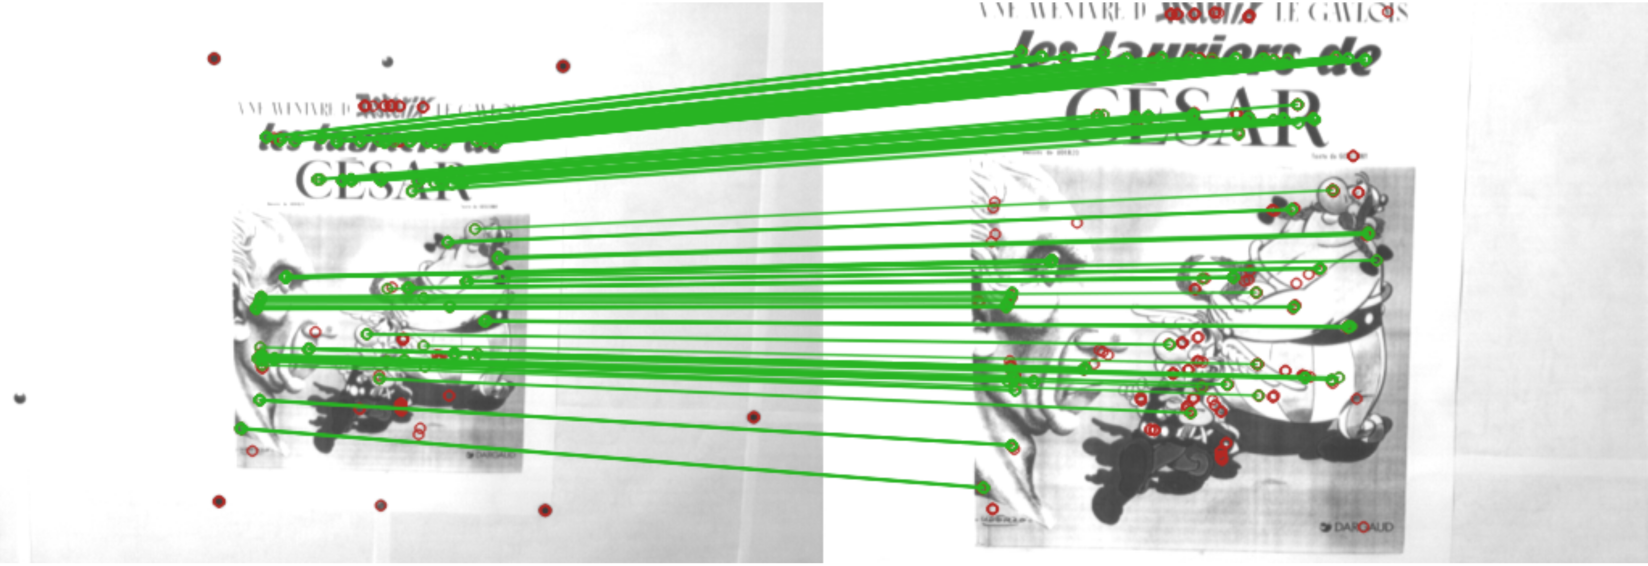
\includegraphics[scale=0.5]{text_img/ex_ASTERIX_MSER_SIFT.pdf}}
	\caption{Transformace zoom ze subsetu Asterix, detektor MSER,
		deskriptor SIFT} \label{ex_asterix}
\end{figure}

\begin{figure}[htp] 
	\centering{
		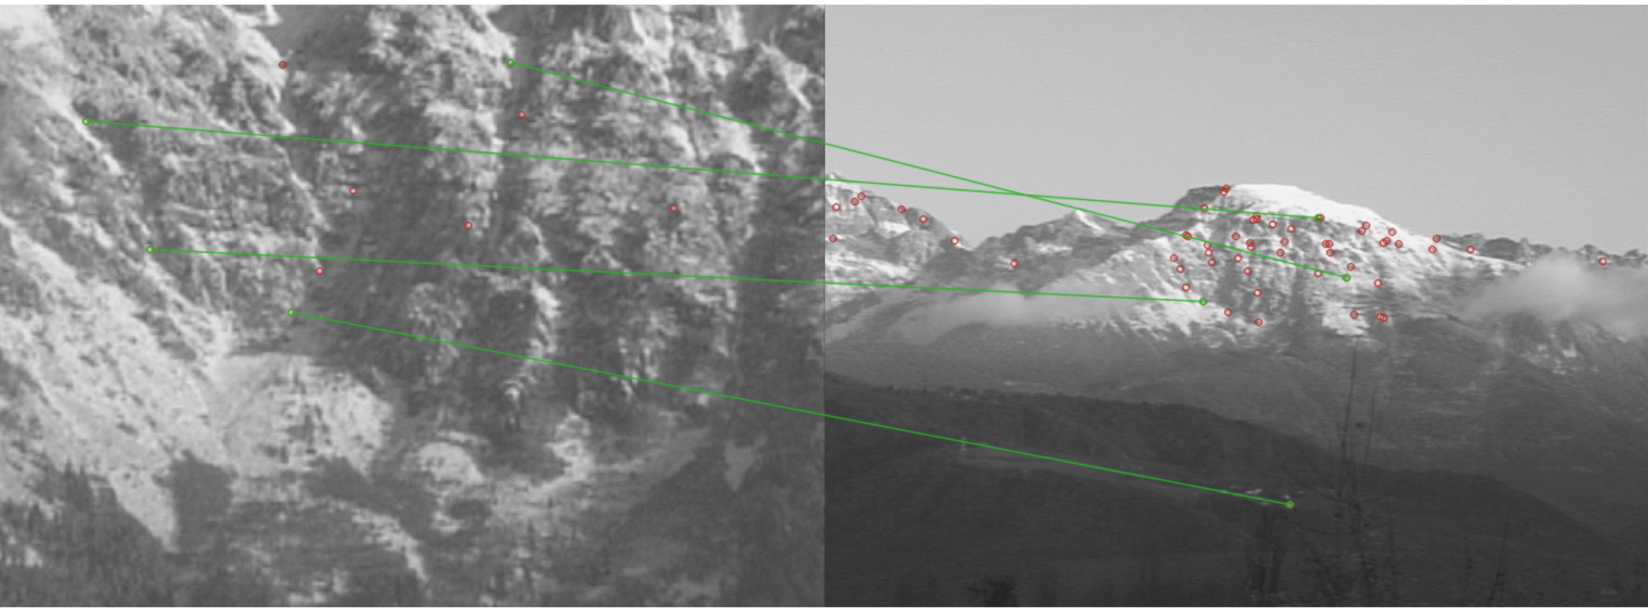
\includegraphics[scale=0.5]{text_img/ex_BELLEDONNE_FAST_ORB.pdf}}
	\caption{Ukázka transformace zoom ze subsetu Belledonne, detektor FAST,
		deskriptor ORB}	\label{ex_belledonne}
\end{figure}

\begin{figure}[htp] 
	\centering{
		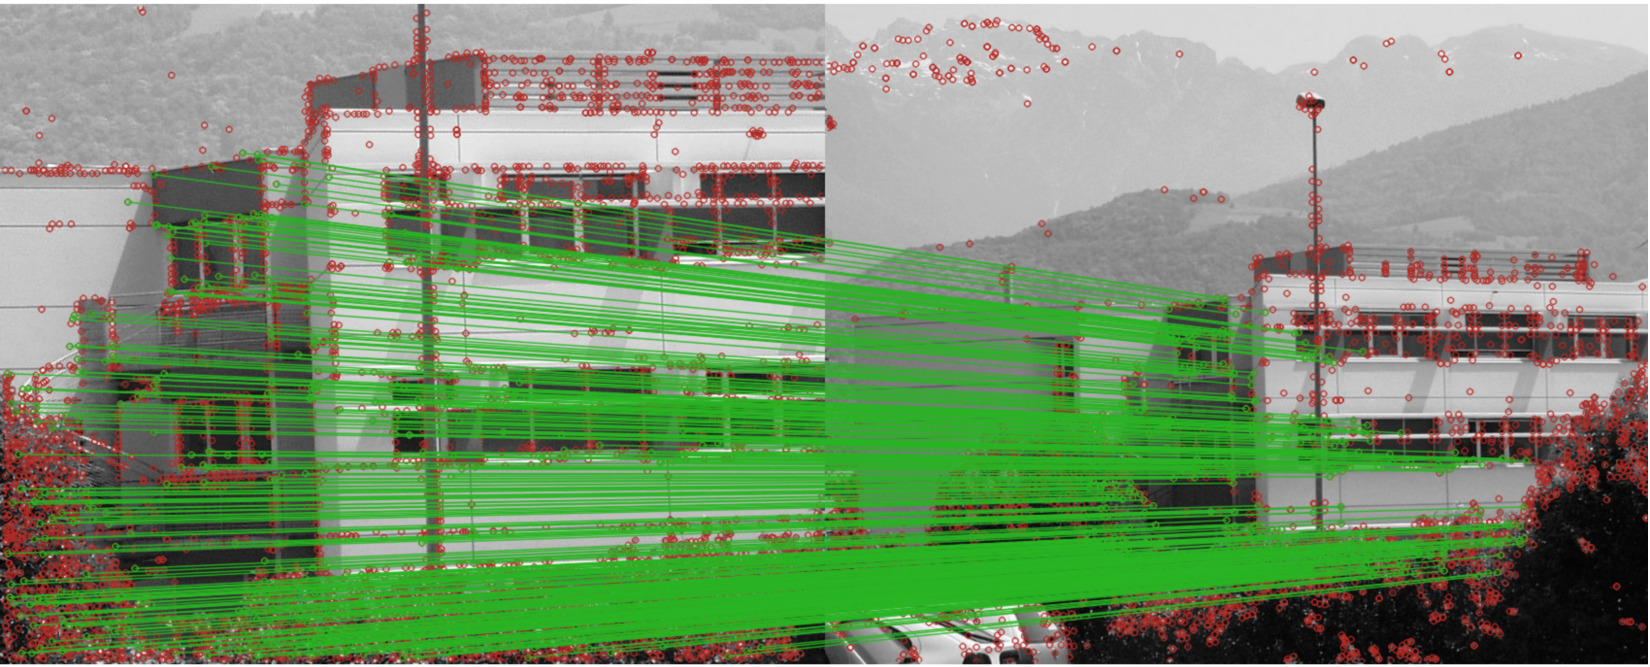
\includegraphics[scale=0.5]{text_img/ex_ENSIMAG_SIFT_SIFT.pdf}}
	\caption{Ukázka transformace zoom ze subsetu Ensimag, detektor i 
		deskriptor SIFT} \label{ex_ensimag}
\end{figure}

\begin{figure}[htp] 
	\centering{
		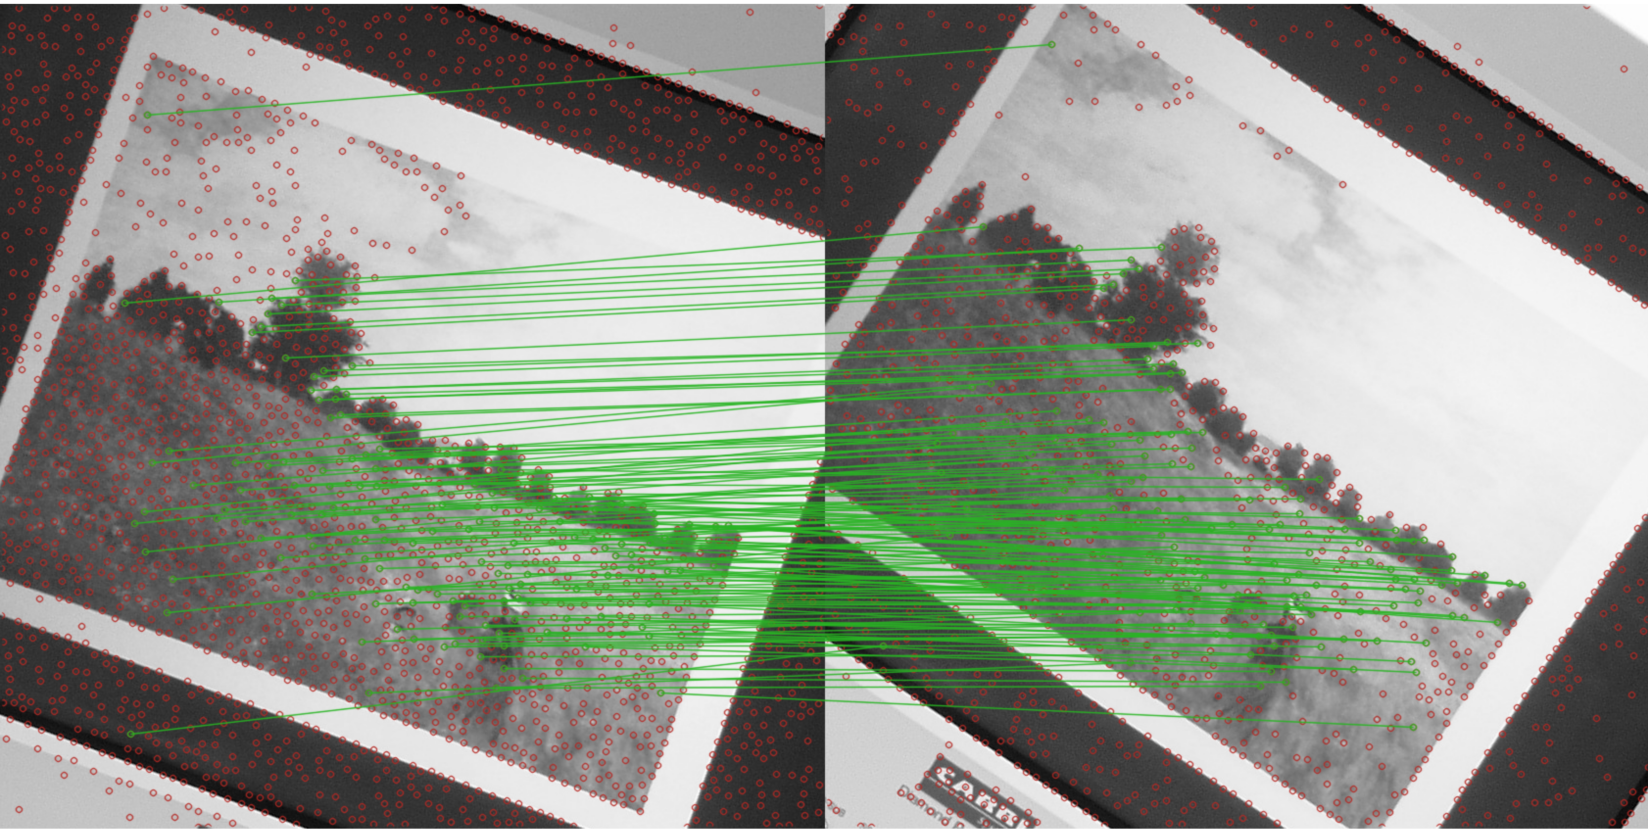
\includegraphics[scale=0.5]{text_img/ex_MONET_GFTT_SIFT.pdf}}
	\caption{Ukázka transformace rotace ze subsetu Monet, detektor GFTT, 
		deskriptor SIFT} \label{ex_MONET}
\end{figure}

\begin{figure}[htp] 
	\centering{
		\includegraphics[scale=0.8]{text_img/Detector_performance.pdf}}
	\caption{Přehled výkonnosti detektorů na jednotlivých datasetech} \label{det_perf}
\end{figure}

\begin{figure}[htp] 
	\centering{
		\includegraphics[scale=0.8]{text_img/Descriptor_performance.pdf}}
	\caption{Přehled výkonnosti deskriptorů na jednotlivých datasetech}	\label{desc_perf}
\end{figure}

\begin{figure}[htp] 
	\centering{}
		\includegraphics[scale=1]{text_img/Det_desc_perf.pdf}
	\caption{Přehled výkonnosti kobinací detektor->deskriptor na jednotlivých datasetech} \label{det_desc_perf}
\end{figure}

V tabulkách \ref{det_perf} a \ref{desc_perf} je uveden přehled celkových průměrných výkonností jednotlivých deskriptorů
a detektorů. Tento přehled je získán vždy testováním uvedeného subsetu uvedenou metodou a všemi
metodami z druhé kategorie. Tedy například skóre deskriptoru SURF je průměrem kombinace
deskriptoru SURF a všech testovaných detektorů na daném datasetu.
Jak je vidět v \ref{det_perf}, v celkové výkonnosti vede detektor ORB. Při bližším pohledu vidíme, že exceluje
zejména na subsetech blur (rozostření), light (změna světelných podmínek) a res (změna rozlišení).
Z toho lze usoudit, že tento detektor založený na algoritmu FAST je vůdči těmto změnám parametrů obrazu
velmi robustní. Za povšimnutí stojí, že jeho varianta - samostatná implementace algoritmu FAST 
v openCV má na všech subsetech asi poloviční hodnocení. Z toho je zřejmé, že se výkonnost detekčního
algoritmu může drasticky změnit drobnými úpravami parametrů a vylepšeními aniž by se změnil jeho princip.
Detektor SURF ve všech disciplínách překonal SIFT, přestože vznikl jako jeho aproximace.

Ve srovnání deskriptorů (tabulka \ref{desc_perf} ) naopak ORB, založený na algoritmu BRIEF zaostává nad svou samostatnou implementací.
Jako deskriptor má SIFT nad SURF převahu ve statických scénářích (subsety blur, light, res).

Ze srovnání kombinací (tabulka \ref{det_desc_perf}) je zřejmé, že všechny detektory mají nejlepší výsledky v kombinaci s deskriptory SIFT a SURF.

Při aplikaci v reálném čase na frekvenci 20Hz je na jeden celý cyklus uvažovaného systému k dispozici 0.05 vteřiny. Uvažujeme-li, že systém musí v každém cyklu provádět i jiné operace než detekci a popis příznaků, můžeme počítat s 0.025 vteřiny pro obě operace dohromady. Časy v tabulkách \ref{det_times} a \ref{desc_times} představují dobu potřebnou pro nalezení příznaků v obou obrazech z testovaného páru, náročnost na jednom obraze bude tedy zhruba poloviční. Do této periody by se podle získaných dat žádná z kombinací zkoumaných metod nevešla. To je pravděpodobně způsobeno nedokonalým nastavením parametrů jednotlivých metod, vysokým rozlišením zpracovávaných obrazů a vysokým množstvím detekovaných příznaků (nebylo nijak omezeno), protože všechny porovnávané metody již byly nějakým způsobem v systémech pracujících v reálném čase nasazeny.

Z porovnání časů potřebných k detekci a popisu příznaků v tabulkách \ref{det_times} a \ref{desc_times} lze vidět, že SIFT a SURF platí za svoji
výkonnost o řád delším časem detekce před ostatními s výjimkou MSER a dokonce o dva řády delším časem výpočtu deskriptorů.

Dle tabulky \ref{match_count} produkuje při daném nastavení největší množství příznaků detektor ORB. Lze ale také vidět, že množství
detekovaných příznaků nemá přímou souvislost s kvalitou aproximace matice homografie.

Grafy \ref{graph_monet} a \ref{graph_asterix} zachycují vývoj kvality aproximace homografie při postupném zpracovávání subsetů Monet a Asterix.
Výsledky odpovídají situaci, kdy dataset Monet sestává z postupné rotace obrazu o 360 stupňů - nejhorší výsledky vykazují metody uprostřed, tedy
v natočení blížícím se 180 stupňům. Dataset Asterix naopak sestává z postupného vzdálení se od zdrojového obrázku, tedy zkoumané páry jsou postupně
náročnější.

\begin{figure}[htp] 
	\centering{
		\includegraphics[scale=0.8]{text_img/Detection_times.pdf}}
	\caption{Přehled průměrné rychlosti detekce jednotlivými metodami ve vteřinách} \label{det_times}
\end{figure}

\begin{figure}[htp] 
	\centering{
		\includegraphics[scale=0.8]{text_img/Description_times.pdf}}
	\caption{Přehled průměrné rychlosti deskripce jednotlivými metodami ve vteřinách} \label{desc_times}
\end{figure}

\begin{figure}[htp] 
	\centering{
		\includegraphics[scale=0.8]{text_img/Match_count.pdf}}
	\caption{Průměrné počty detekovaných a přiřazených příznaků jednotlivými kombinacemi metod}	\label{match_count}
\end{figure}


\begin{figure}[htp] 
	\centering{
		\includegraphics[scale=0.8]{text_img/graph_monet.pdf}}
	\caption{Kvalita odhadu homografie na párech obrázků ze subsetu Monet (rotace)}	\label{graph_monet}
\end{figure}

\begin{figure}[htp] 
	\centering{
		\includegraphics[scale=0.8]{text_img/graph_asterix.pdf}}
	\caption{Kvalita odhadu homografie na párech obrázků ze subsetu Asterix (zoom)}	\label{graph_asterix}
\end{figure}